\cotefile{104}
\scanpage{2}

\figure{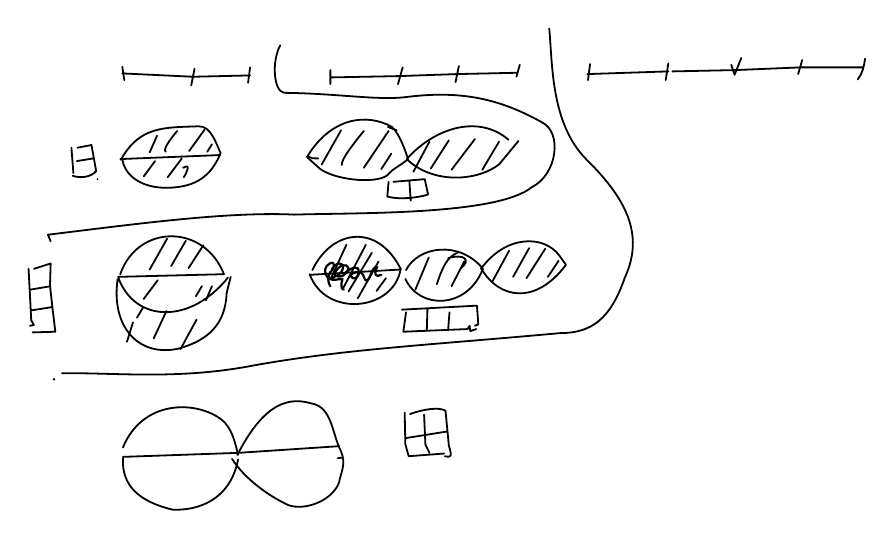
\begin{tikzpicture}[x=.0085cm,y=-.0085cm,line width=.65pt,line cap=round,line join=round]
% Three marked segments across the top.
\draw (227,131)--(333,136)--(418,134) (227,121)--(230,141) (335,124)--(330,149) (418,122)--(415,145);
\draw (538,137)--(641,135)--(727,132)--(818,130) (538,126)--(538,147) (646,122)--(639,147) (730,120)--(725,144) (821,118)--(816,136);
\draw (922,132)--(1043,128) (1049,128)--(1144,126)--(1240,122)--(1334,122) (926,117)--(923,141) (1043,116)--(1039,141) (1137,118)--(1142,133)--(1152,108) (1243,111)--(1237,132) (1337,109) .. controls (1335,122) and (1333,131) .. (1326,140);
% The long dividers pass between the groups of figures.
\draw (463,89) .. controls (450,113) and (453,158) .. (469,160)
 .. controls (552,161) and (610,172) .. (654,166)
 .. controls (736,156) and (793,170) .. (854,204)
 .. controls (885,219) and (877,282) .. (839,301)
 .. controls (787,343) and (583,339) .. (484,342)
 .. controls (384,337) and (240,357) .. (116,372)--(120,382);
\draw (865,64) .. controls (870,116) and (867,205) .. (920,259)
 .. controls (979,317) and (1008,371) .. (978,436)
 .. controls (957,497) and (929,519) .. (882,519)
 .. controls (685,537) and (557,543) .. (420,568)
 .. controls (309,589) and (217,578) .. (137,579);
\fill (125,588) circle[radius=2.2];
% Upright two-cell strip and bisected, hatched oval.
\draw (151,242)--(154,280) (160,242)--(181,238)--(188,277) .. controls (182,284) and (168,289) .. (153,284)
 (159,262)--(184,258);
\fill (190,289) circle[radius=1.45];
\draw (225,260) .. controls (253,209) and (291,212) .. (341,210)
 .. controls (360,209) and (368,238) .. (374,250)
 .. controls (357,292) and (328,301) .. (294,302)
 .. controls (255,302) and (231,284) .. (227,259);
\draw (224,259)--(373,253);
\draw (279,224)--(268,249) (309,217)..controls(299,229)and(287,245)..(292,248)
 (350,215)--(327,247) (361,237)--(354,248)
 (276,262)--(259,285) (316,258)--(295,286) (318,272)..controls(331,264)and(322,282)..(319,286);
% Two joined lenses, above a two-cell strip.
\draw (503,256) .. controls (539,196) and (593,190) .. (630,211)
 .. controls (641,221) and (650,246) .. (654,259)
 .. controls (641,270) and (632,273) .. (626,280)
 .. controls (615,297) and (549,292) .. (523,274)--(503,256);
\draw (504,255)..controls(508,258)and(513,258)..(520,258);
\draw (637,216)--(624,211)
 (652,259) .. controls (696,210) and (761,193) .. (804,230)
 (652,259) .. controls (690,296) and (756,293) .. (790,267)--(819,232);
\draw (554,216)--(525,267) (588,217)..controls(570,239)and(554,260)..(555,268)
 (625,217)--(588,272) (629,251)--(614,274)
 (686,233)--(662,278) (715,231)--(688,273) (754,229)--(719,275) (790,233)--(765,275);
\draw (625,293)--(623,315)..controls(641,320)and(668,317)..(684,312)--(679,289)--(632,293)
 (656,292)--(658,321);
% Three-cell strip, oval and additional lower boundary.
\draw (87,423)--(91,500)--(95,507)--(89,508)
 (95,423)--(120,415)--(119,448)--(123,484)--(127,517)--(93,518)
 (90,454)--(120,449) (92,485)--(123,480);
\draw (224,431) .. controls (250,356) and (349,355) .. (379,431)
 (221,435)--(379,431)
 (221,436) .. controls (246,504) and (329,506) .. (385,436)
 (220,439) .. controls (210,509) and (251,556) .. (312,542)
 .. controls (357,529) and (381,505) .. (383,459)--(389,435);
\draw (294,378)--(268,424) (322,381)--(300,419) (348,388)--(326,422)
 (280,440)--(259,468) (346,449)--(337,464) (361,449)--(352,470)
 (258,481)--(249,496) (243,503)--(234,532) (293,486)--(274,527) (338,499)--(314,543);
% Three horizontal lenses. The first contains heavily retraced ink.
\draw (511,425) .. controls (540,364) and (608,354) .. (643,423);
\draw (643,423) .. controls (633,486) and (531,497) .. (507,431);
\draw (507,432)--(643,424);
\draw (562,387)--(538,439) (591,387)--(556,454) (600,399)--(565,457)
 (610,412)--(579,467) (621,437)--(607,456);
% Dense retraced loops on the chord; no recoverable word or defensible word count.
% Whether an earlier written label was cancelled here remains uncertain.
\draw[line width=.8pt]
 (535,437) .. controls (527,429) and (529,419) .. (537,415)
 .. controls (547,410) and (544,424) .. (537,429)
 .. controls (534,436) and (534,444) .. (538,449)
 (540,424) .. controls (547,412) and (557,413) .. (557,421)
 .. controls (555,432) and (544,436) .. (537,437)
 .. controls (541,442) and (549,438) .. (556,438)
 .. controls (554,446) and (553,453) .. (558,454)
 (544,430) .. controls (551,416) and (563,414) .. (565,422)
 .. controls (565,431) and (551,439) .. (544,432)
 (559,430) .. controls (571,419) and (582,418) .. (580,428)
 .. controls (579,438) and (572,441) .. (568,433)
 .. controls (570,427) and (586,426) .. (587,432)
 .. controls (591,445) and (593,443) .. (598,432)
 .. controls (600,426) and (603,420) .. (608,420)
 .. controls (601,432) and (607,436) .. (614,432);
\draw (651,425)..controls(669,389)and(731,380)..(766,423)
 ..controls(742,484)and(671,484)..(650,438);
\draw (685,406)--(665,454) (728,399)..controls(712,405)and(705,422)..(697,446)
 (714,407)..controls(738,400)and(749,410)..(733,422) (738,412)--(719,449);
\draw (763,423)..controls(800,372)and(857,372)..(880,403)--(890,417)
 ..controls(846,476)and(791,470)..(763,422);
\draw (805,396)--(780,442) (835,392)--(811,435) (859,393)--(831,437) (879,411)--(863,435);
\draw (645,484)--(757,478)--(759,506)--(754,508)
 (651,488)--(647,517)--(743,513)--(746,508)--(747,516)--(756,513) (683,484)--(682,516) (716,488)--(714,513);
% Unshaded pair with one through-line and a four-cell square.
\draw (228,690)..controls(257,619)and(336,619)..(375,648)
 ..controls(390,660)and(395,679)..(400,701);
\draw (400,708) ..controls(391,756)and(356,784)..(303,783)
 ..controls(252,771)and(226,747)..(228,706);
\draw (399,701)..controls(432,637)and(466,611)..(509,624)
 ..controls(541,629)and(540,669)..(554,696)
 ..controls(562,715)and(553,729)..(551,742)
 ..controls(541,770)and(499,785)..(475,776)
 ..controls(447,763)and(411,738)..(391,707);
\draw (228,704)--(400,698)--(551,688);
\draw (556,705)--(549,706);
\draw (649,638)--(650,685)--(655,703)--(708,699)
 (657,640)..controls(676,633)and(700,629)..(710,635)--(715,687)
 ..controls(720,704)and(719,705)..(709,703)
 (678,641)--(680,686)--(686,698) (650,676)--(713,666);
\end{tikzpicture}}

\[
(\text{Ss sets})\,\hookleftarrow\,
(\mathrm{Cat})\,
\unsure{\hookleftarrow|\deleted{\supset}\hookleftarrow}\,
(\deleted{\unsure{\mathrm{Ord}}}\unsure{\text{Préord}|\text{PréOrd}})\,
\supset\,(\mathrm{Ord})\,\supset\,
\left(\overset{\inserted{\text{Maquettes}}}{\deleted{\text{Triang}}}\right)
\]
% The second link is certainly hooked and left-pointing. Its alternative concerns
% only the possible earlier inclusion stroke, not the live arrow's shape.

\[
Fx\longrightarrow Fy
\]

\[
\underset{\smile}{x}\leq\underset{\smile}{y}
\]

% Lower-right margin: six small dark nonlinguistic marks; their origin is uncertain.
\margin{\figure{
\begin{tikzpicture}[x=.025cm,y=-.025cm,line cap=round,line join=round]
\fill (7,5) .. controls (10,4) and (12,3) .. (16,2)
 -- (9,7) .. controls (8,8) and (10,9) .. (10,11)
 .. controls (8,14) and (5,9) .. (7,5) -- cycle;
\fill (9,17) .. controls (12,15) and (13,17) .. (13,18)
 .. controls (17,20) and (13,22) .. (9,21) -- cycle;
\fill (5,27) ellipse[x radius=1.3,y radius=.9];
\fill (2,35) circle[radius=1.3];
\fill (15,35) .. controls (13,36) and (9,38) .. (10,41)
 .. controls (11,43) and (14,45) .. (14,45)
 .. controls (18,46) and (15,42) .. (14,40)
 .. controls (13,38) and (17,36) .. (15,35) -- cycle;
\fill (13,68) ellipse[x radius=2.2,y radius=2.8];
\end{tikzpicture}}}
% archive sheet number: 1

\scanpage{3}

\noindent\begin{minipage}[t]{.34\linewidth}
\(\checkmark\)
\diagram{\begin{tikzcd}[ampersand replacement=\&,column sep=1.5em]
{\unsure{F|\mathbb F}}_0
 \& \mathbb F_1 \arrow[l,shift right=.7ex,"s_1"'] \arrow[l,shift left=.7ex,"t_1"]
 \& \mathbb F_2\mathord{.} \arrow[l,shift right=.7ex,"s_2"'] \arrow[l,shift left=.7ex,"t_2"]
\end{tikzcd}}
\diagram{\begin{tikzcd}[ampersand replacement=\&,column sep=1.5em]
\mathbb F_0 \arrow[r,dash,"\sigma_1", "{\unsure{\cdot|\scriptscriptstyle >}}" description,pos=.97]
 \& f_1 \arrow[r,"\sigma_2"]
 \& F_2
\end{tikzcd}}
\[
\mu^4_1\quad\mu^2_1\quad\mu^2_2
\]
\[
\begin{aligned} &a\\ &\ell\\\ &r\end{aligned}
\]
\end{minipage}\hfill
\begin{minipage}[t]{.64\linewidth}
\figure{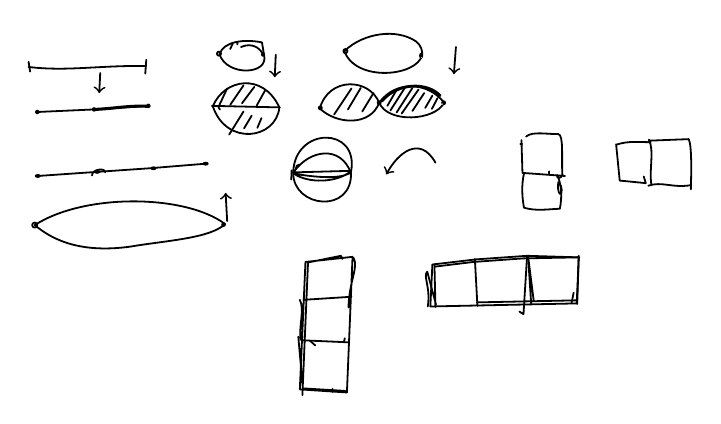
\begin{tikzpicture}[x=.0065cm,y=-.0065cm,line width=.65pt,line cap=round,line join=round]
\draw (723,94)..controls(797,103)and(858,91)..(953,92)
 (723,84)--(726,103) (953,80)--(951,107);
\draw[->] (863,106)--(861,145);
\draw (740,182)--(851,177)--(957,170);
\foreach \x/\y in {740/182,851/177,957/170}{\fill (\x,\y) circle[radius=4.4];}
\draw[line width=1.1pt] (852,177)..controls(895,175)and(917,169)..(958,171);
\draw (1096,69)..controls(1104,44)and(1144,39)..(1179,46)--(1183,70)
 ..controls(1194,110)and(1110,113)..(1096,69);
\draw (1138,55)..controls(1159,46)and(1174,56)..(1181,69);
\draw (1122,48)--(1117,59) (1131,46)--(1131,50);
\draw (1095,68) circle[radius=4];\fill (1181,70) circle[radius=4];
\draw[->] (1206,70)--(1204,114);
\draw (1083,171)..controls(1105,117)and(1181,104)..(1213,173)
 ..controls(1207,235)and(1110,250)..(1083,171);
\draw (1081,170)--(1214,173);
\draw (1111,136)--(1096,168)..controls(1093,172)and(1094,175)..(1097,177) (1143,130)--(1117,168) (1164,133)--(1140,165)
 (1185,140)--(1169,169) (1143,181)--(1115,226) (1159,189)--(1144,214) (1178,194)--(1170,213);
\draw (1340,63)..controls(1379,26)and(1443,19)..(1480,44)
 ..controls(1490,52)and(1493,63)..(1492,71)
 ..controls(1481,113)and(1362,124)..(1340,63);
\draw (1342,63) circle[radius=4];\fill (1490,72) ellipse[x radius=4,y radius=6];\fill[white] (1490.8,75.5) circle[radius=.9];
\draw[->] (1558,55)--(1554,108);
\draw (1292,175)..controls(1310,112)and(1389,116)..(1408,164)
 ..controls(1391,210)and(1325,207)..(1292,175);
\draw (1408,164)..controls(1440,119)and(1504,123)..(1535,164)
 ..controls(1517,199)and(1426,205)..(1408,164);
\draw[line width=1pt] (1413,161)..controls(1445,123)and(1503,124)..(1527,150);
\foreach \x/\y in {1293/174,1408/164}{\fill (\x,\y) circle[radius=4.8];}\fill (1534,164) circle[radius=4.8];\fill[white] (1531.5,166.5) circle[radius=1.2];
\draw (1354,136)--(1320,187) (1372,135)--(1347,177) (1397,145)--(1375,181)
 (1442,139)--(1424,170) (1458,135)--(1430,179) (1473,135)--(1442,183)
 (1485,138)--(1452,185) (1496,145)--(1473,180) (1512,150)--(1498,174) (1522,155)--(1511,176);
\draw (741,307)--(857,299)--(959,292)--(1069,283);
\foreach \x/\y in {741/307,857/299,967/292,1069/283}{\fill (\x,\y) ellipse[x radius=6,y radius=3.8];}
\draw (847,306)..controls(846,294)and(873,290)..(873,300);
\draw (735,403)..controls(833,340)and(1030,343)..(1107,401)
 ..controls(1077,429)and(993,433)..(922,445)
 ..controls(814,460)and(762,425)..(735,403);
\draw (735,403) circle[radius=5];
\fill (1104,402) circle[radius=4.6];
\draw[->] (1111,395)--(1108,340);
\draw (1240,301)..controls(1242,210)and(1370,209)..(1353,299)
 ..controls(1357,382)and(1240,370)..(1240,301);
\draw (1241,299)..controls(1274,254)and(1332,248)..(1352,299)
 (1240,300)--(1352,297) (1242,303)..controls(1271,322)and(1324,320)..(1351,299)
 (1244,303)..controls(1288,310)and(1328,313)..(1350,302);
\draw (1245,294)..controls(1245,289)and(1248,284)..(1251,285)
 (1237,296)..controls(1239,302)and(1235,307)..(1236,314);
\draw[->] (1518,281)..controls(1487,226)and(1444,263)..(1422,304);
\draw (1686,237)--(1688,301)--(1771,307)
 (1695,230)..controls(1707,219)and(1739,226)..(1758,225)
 ..controls(1769,227)and(1764,273)..(1766,305)
 (1740,302)--(1740,298)
 (1691,302)..controls(1686,324)and(1687,348)..(1691,369)
 ..controls(1715,376)and(1736,372)..(1761,371)
 ..controls(1766,347)and(1764,323)..(1756,305);
\draw (1683.8,244.5)--(1687.5,244.5)
 (1756,306)..controls(1753,311)and(1764,313)..(1765,306)
 (1758,319)..controls(1768,328)and(1765,343)..(1761,342)..controls(1757,337)and(1757,328)..(1758,319);
\draw (1871,245)--(1878,316)--(1929,321)--(1925,308)
 (1871,246)..controls(1894,238)and(1917,241)..(1938,241)
 (1935,236)..controls(1946,257)and(1935,296)..(1940,325)
 (1937,238)--(2013,235)..controls(2019,250)and(2018,298)..(2017,333)
 (1934,326)..controls(1961,317)and(1980,331)..(2017,325);
\draw (1264,475)--(1356,465)--(1345,730)--(1253,724)--cycle
 (1260,549)--(1354,543) (1256,628)--(1348,632)
 (1258,735)--(1269,476)--(1333,463)--(1336,469)
 (1358,467)..controls(1368,486)and(1350,509)..(1348,564)
 (1253,549)..controls(1263,567)and(1250,604)..(1255,627)
 (1250,621)--(1259,722)--(1342,727);
\draw (1273,629)--(1283,638) (1339,632)--(1341,624)
 (1317,729)--(1317,723);
\draw (1512,480)--(1597,470)--(1697,463)--(1798,466)--(1794,556)--(1508,562)--cycle
 (1595,469)--(1600,561) (1697,464)--(1690,577)--(1682,572);
\draw (1518,484)--(1592,475)--(1690,468)--(1799,466)
 (1503,562)..controls(1509,524)and(1493,502)..(1502,494)--(1519,558)
 (1518,563)--(1516,480) (1599,554)--(1794,550) (1705,556)--(1699,464)--(1710,551)
 (1784,555)--(1788,535) (1795,557)--(1798,463);
\end{tikzpicture}}
\end{minipage}

% printed form
% Typed address label, running from the bottom toward the top of the sheet.
\noindent\texttt{MR\quad LE PROFESSEUR GROTHENDIECK ALEX.}\\
\texttt{MATHEMATIQUES\unsure{.}\hspace{8em}5}

\[
I_A\,\circ\,\unsure{S|s}\longrightarrow S
\]

\figure{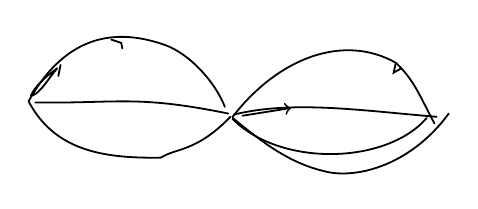
\begin{tikzpicture}[x=.014cm,y=-.014cm,line width=.65pt,line cap=round]
\draw (265,1054)..controls(300,991)and(347,988)..(389,1003)
 ..controls(411,1011)and(434,1036)..(443,1059);
\draw (448,1068)..controls(417,1100)and(399,1096)..(385,1105)
 ..controls(329,1106)and(288,1097)..(265,1054);
\draw (271,1055)..controls(347,1056)and(362,1048)..(446,1065);
\draw (450,1068)..controls(491,1015)and(550,992)..(598,1019)
 ..controls(615,1035)and(620,1050)..(633,1074)
 (646,1065)..controls(610,1114)and(559,1125)..(532,1117)
 ..controls(498,1109)and(471,1086)..(450,1069);
\draw (451,1066)..controls(504,1053)and(564,1062)..(635,1068)
 (450,1070)..controls(494,1114)and(590,1111)..(626,1069);
\draw[->] (459,1067)--(503,1060);
% Small contour returns; their semantic status as arrows is not asserted.
\draw (267,1049)..controls(275,1048)and(283,1033)..(291,1024)
 (291,1024)..controls(280,1032)and(271,1040)..(267,1049)
 (294,1021)--(292,1031)
 (340,998)--(349,1001)--(350,1006)
 (598,1019)--(596,1028)--(603,1024);
\end{tikzpicture}}

\figure{\begin{tikzpicture}[x=.011cm,y=-.011cm,line width=.65pt,line cap=round]
\draw (1326,876)..controls(1346,861)and(1385,870)..(1418,869)--(1439,944)
 (1331,884)--(1345,942)..controls(1348,950)and(1384,947)..(1402,949)--(1398,943)
 (1424,859)--(1515,854)..controls(1535,874)and(1536,912)..(1538,945)
 (1408,956)..controls(1444,943)and(1500,953)..(1542,939)
 (1343,947)..controls(1346,970)and(1348,992)..(1361,1013)
 ..controls(1396,1033)and(1419,1029)..(1445,1016)--(1548,1012)--(1541,944)
 (1435,949)--(1444,1019) (1444,957)--(1445,1011) (1538,998)--(1541,1012);
\fill (1316,870) circle[radius=1.5];\fill (1738,730) circle[radius=1.1];
\draw (1725.7,731)--(1730,731);
\draw (1711,748)--(1725,862) (1716,713)--(1734,775)
 (1709,763)--(1843,753)--(1939,748)--(2043,744)--(2167,739)
 (1725,760)--(1834,762)
 (1838,737)--(1845,770) (1935,735)--(1942,760)
 (2041,735)--(2047,752) (2153,730)--(2153,756) (2163,735)--(2162,746);
\end{tikzpicture}}

\[
\Delta_{n_1}\times\Delta_{n_2}\times
\mathord{-}\,\mathord{-}\,\unsure{<|\times}\,\Delta_{n_n}
\]

\figure{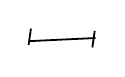
\begin{tikzpicture}[line width=.65pt]
\draw (0,0)--(.85,.04) (0,-.05)--(.03,.16) (.81,-.08)--(.84,.13);
\end{tikzpicture}}

\diagram{\begin{tikzcd}[ampersand replacement=\&,column sep=1.4em,row sep=1em,cells={nodes={inner sep=.4pt}}]
\bullet\arrow[r]\arrow[d,shorten >=3pt] \& {}\arrow[r] \& {}\arrow[r] \& {}\arrow[r] \& \bullet\\
\bullet \& \& \& \&
\end{tikzcd}}

\[
\Delta_{n_1}\times\Delta
\]

\noindent\begin{minipage}{.40\linewidth}
\diagram{\begin{tikzcd}[ampersand replacement=\&,column sep=1.4em,row sep=1.2em,cells={nodes={inner sep=0pt,minimum size=0pt}},
 execute at end picture={\foreach \rowa/\rowb in {1/2,2/3,3/4}{
 \foreach \fracx/\fracy/\low/\high in {.04/.37/.12/.97,.24/.68/.03/.89,.62/.93/.16/.77}{
 \path (\tikzcdmatrixname-\rowb-1.center)--(\tikzcdmatrixname-\rowb-2.center) coordinate[pos=\fracx] (hatchlo);
 \path (\tikzcdmatrixname-\rowa-1.center)--(\tikzcdmatrixname-\rowa-2.center) coordinate[pos=\fracy] (hatchhi);
 \path (hatchlo)--(hatchhi) coordinate[pos=\low] (inklo) coordinate[pos=\high] (inkhi);
 \draw[line width=.33pt] (inklo)--(inkhi);}}}]
{}\arrow[r]\arrow[d,dash] \& {}\arrow[r]\arrow[d,dash] \& {}\arrow[r]\arrow[d,dash] \& {}\arrow[r]\arrow[d,dash] \& {}\arrow[d,dash]\\
{}\arrow[r]\arrow[d,dash] \& {}\arrow[r]\arrow[d,dash] \& {}\arrow[r]\arrow[d,dash] \& {}\arrow[r]\arrow[d,dash] \& {}\arrow[d,dash]\\
{}\arrow[r]\arrow[d,dash] \& {}\arrow[r]\arrow[d,dash] \& {}\arrow[r]\arrow[d,dash] \& {}\arrow[r,shorten <=2pt,shorten >=2pt]\arrow[d,dash] \& {}\arrow[d,dash]\\
{}\arrow[r] \& {}\arrow[r] \& {}\arrow[r] \& {}\arrow[r,shorten <=2pt,shorten >=2pt] \& {}
\arrow[from=1-1,to=2-2,draw=none,"\Downarrow" description]
\arrow[from=1-2,to=2-3,draw=none,"\Downarrow" description]
\arrow[from=1-3,to=2-4,draw=none,"\Downarrow" description]
\arrow[from=1-4,to=2-5,draw=none,"\Downarrow" description]
\arrow[from=2-1,to=3-2,draw=none,"\Downarrow" description]
\arrow[from=2-2,to=3-3,draw=none,"\Downarrow" description]
% The middle-row third cell has two heavy descending strokes, no secure head.
\arrow[from=2-3,to=3-4,draw=none,"{\vcenter{\hbox{\begin{tikzpicture}[x=.55em,y=.55em,line width=.65pt]\draw (0,1.1)--(0,0) (.23,1.1)--(.23,0);\end{tikzpicture}}}}" description]
\arrow[from=2-4,to=3-5,draw=none,"\Downarrow" description]
\arrow[from=3-1,to=4-2,draw=none,"\Downarrow" description]
\arrow[from=3-2,to=4-3,draw=none,"\Downarrow" description]
\arrow[from=3-3,to=4-4,draw=none,"\Downarrow" description]
\arrow[from=3-4,to=4-5,draw=none,"\Downarrow" description]
\arrow[from=1-1,to=4-1,shift left=.22ex,shorten >=4pt]
\arrow[from=1-2,to=4-2,dash,shift right=.3ex]
\arrow[from=1-3,to=4-3,dash,shift right=.3ex]
\arrow[from=1-4,to=4-4,dash,shift right=.3ex]

\end{tikzcd}}
\end{minipage}\hfill
\begin{minipage}{.58\linewidth}
\figure{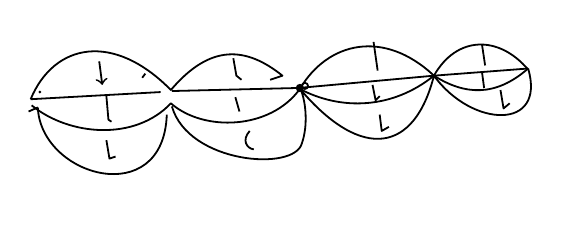
\begin{tikzpicture}[x=.013cm,y=-.013cm,line width=.65pt,line join=round]
\draw (1010,1405)..controls(1033,1350)and(1091,1339)..(1147,1396)
 ..controls(1186,1350)and(1221,1354)..(1256,1382)--(1244,1386)
 (1273,1395)..controls(1300,1349)and(1355,1336)..(1404,1382)
 ..controls(1426,1343)and(1467,1342)..(1496,1376);
\draw (1010,1405)--(1137,1398)
 (1148,1397)--(1272,1394)--(1404,1382)--(1496,1375);
\fill (1019,1398) circle[radius=1.5];
\draw (1122,1380)--(1119,1384)
 (1008,1417)--(1017,1413);
\draw (1278,1392) circle[radius=3];
\draw (1011,1411)..controls(1048,1441)and(1112,1446)..(1147,1409)
 ..controls(1179,1437)and(1244,1435)..(1273,1395)
 ..controls(1313,1416)and(1363,1415)..(1404,1382)
 ..controls(1434,1401)and(1464,1403)..(1496,1375);
\draw (1017,1413)..controls(1020,1481)and(1140,1514)..(1143,1420)
 (1148,1412)..controls(1164,1468)and(1268,1476)..(1275,1448)
 ..controls(1281,1431)and(1279,1408)..(1274,1396)
 ..controls(1334,1466)and(1385,1457)..(1404,1382)
 ..controls(1441,1433)and(1514,1436)..(1496,1375);
\fill (1273,1394) circle[radius=4];
\draw[->] (1077,1368)--(1080,1391);
\draw (1084,1402)--(1086,1425)--(1089,1427) (1084,1445)--(1087,1463)--(1093,1461)
 (1208,1365)--(1211,1382)--(1216,1386) (1210,1403)--(1214,1417)
 (1224,1436)..controls(1216,1445)and(1221,1453)..(1228,1454)
 (1345,1349)--(1349,1377) (1344,1391)--(1347,1406)--(1351,1402)
 (1351,1420)--(1353,1436)--(1360,1432)
 (1451,1352)--(1454,1372) (1451,1379)--(1453,1394)
 (1469,1396)--(1472,1414)--(1478,1409);
\end{tikzpicture}}
\end{minipage}

\[
\vcenter{\hbox{
\begin{tikzpicture}[x=.85em,y=.85em,line width=.38pt,baseline]\draw (0,0)--(.59,.92)--(.82,0)--cycle;\draw (.09,.03)--(.69,.96);\end{tikzpicture}}}_n\times\vcenter{\hbox{
\begin{tikzpicture}[x=.85em,y=.85em,line width=.38pt,baseline]\draw (0,0)--(.59,.92)--(.82,0)--cycle;\draw (.09,.03)--(.69,.96);\end{tikzpicture}}}_{n'}
\]
\[
\begin{aligned}
\mathbb F_0 &= \mathrm{Ob}\,\Delta_{\unsure{kn'|n\,n'|n'}}\\
F_1 &= \deleted{\unsure{\mathrm{Ob}\,\Delta_n|\mathrm{O}\Delta_n}}\deleted{\unsure{\mathrm{Ob}}}{\unsure{\mathbb F|F}}\mathrm{l}^{\unsure{\prime}}(\Delta_n)\times\mathrm{Ob}\,\Delta_{n'}\\
F &\mathrel{\unsure{-|=}} \mathbb F\mathrm{l}\,(\Delta_n)\times\mathbb F\mathrm{l}\,\Delta_{n''})
\end{aligned}
\]
% The detached stroke after live l is prime-like; an isolated pen mark remains possible.
% The lower line has no visible subscript after the initial F and only one visible relation bar.
% The second closing parenthesis has no visible matching opening parenthesis.
% A separate long ink stroke runs toward the right edge beneath the end of this line.
\figure{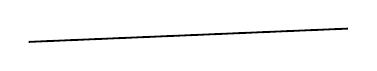
\begin{tikzpicture}[x=.013cm,y=-.013cm,line width=.65pt]
\draw (2040,1652)--(2352,1639);
\end{tikzpicture}}
% archive sheet number: 2

\scanpage{4}

\diagram{\begin{tikzcd}[ampersand replacement=\&,column sep=1.6em,row sep=1.2ex]
\mathrm{Ob}\,C_4
 \arrow[rr,phantom,"{\tikz[baseline=(current bounding box.center),x=.008cm,y=-.008cm,line cap=round,line join=round]{
  \draw[line width=.8pt] (606,136)--(855,170)--(1027,176);
  \draw[line width=.35pt] (611,163)..controls(650,135)and(850,125)..(1023,174)
   (609,137)--(659,146)--(996,171) (607,136)--(617,145)
   (839,165)--(864,184)
   (844,169)..controls(903,188)and(974,188)..(1021,178)
   (998,151)--(1026,174)--(978,193)
   (994,162)--(1025,173)--(964,203);
  \fill (950,130) circle[radius=1.3];
  \fill (999,162)--(1031,172)--(1008,187)--(1013,174)--cycle;
 }}" description,pos=.54] \& \& \tikz[baseline=(targetF.base)]{
 \node[inner sep=0pt] (targetF) {\(\mathrm{Fl}_0\)};
 \fill ([xshift=-.13em,yshift=.02em]targetF.south west) circle[radius=.025em];}
 (\ell_{\unsure{n|1}})\\
{\tikz[baseline=(topproduct.base)]{
 \node[inner sep=0pt] (topproduct) {\(\bigl(\mathbb F\mathrm l\,C_1\times\mathrm{Ob}\,C_2\bigr)\)};
 \fill ([xshift=1.05em,yshift=-.48em]topproduct.west) circle[radius=.025em];}}
 \arrow[u,phantom,"{\tikz[baseline=(current bounding box.center),x=.008cm,y=-.008cm,line cap=round,line join=round]{
  \draw[line width=.45pt] (286,260)--(289,178) (276,208)--(289,178)--(298,199)
   (284,254)..controls(282,246)and(284,202)..(287,185)
   (286,260)--(292,257) (321,257)--(318,184) (321,257)--(327,254)
   (307,190)--(327,173)--(334,182);
 }}" description,pos=.5]
 \& {\begin{aligned}
 &\deleted{\amalg}\;\deleted{\unsure{\mathrm{Fl}_0 C_1\times}}\\[-.3ex]
 &\qquad\inserted{\mathbb F\mathrm l_0(\ell_1)
 \mathbin{\tikz[baseline=(replacementcross.base)]{
  \node[inner sep=0pt] (replacementcross) {\(\times\)};
  \fill ([xshift=.09em,yshift=.12em]replacementcross.north east) circle[radius=.025em];}}
 \mathrm{Ob}\,C_2}
 \end{aligned}} \&
\end{tikzcd}}
% The heavy arrow certainly points right. Its multiple shafts and left spur
% are traced without asserting a separately cancelled earlier left arrow.
% Detached points have unassigned origin/function; the right upward head is gapped.

\[
\mathbb F\mathrm l\,C_{\deleted{\unsure{2}}\unsure{1|2}}\times
\mathbb F\mathrm l(C_2)\times\deleted{\unsure{F|\mathrm{Fl}}}\mathrm{Ob}\,C_3
\]

\figure{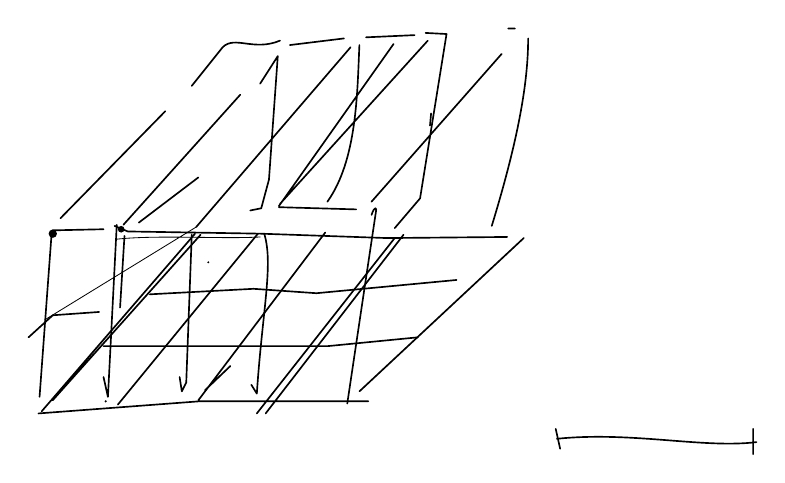
\begin{tikzpicture}[x=.014cm,y=-.014cm,line width=.6pt,line cap=round,line join=round]
\draw (1305,284)--(1351,283) (1361,280)--(1373,285)--(1493,287)--(1608,291)--(1717,290)
 (1304,286)--(1293,435) (1363,279)--(1355,435)--(1351,417) (1370,289)--(1366,354)
 (1431,288)--(1426,422)--(1422,430)--(1420,417)
 (1497,288)..controls(1505,316)and(1495,357)..(1490,432)--(1485,424)
 (1594,270)..controls(1597,261)and(1599,264)..(1598,267)--(1572,441);
\draw[line width=.3pt] (1298,365)--(1435,281)
 (1363,292)..controls(1400,288)and(1460,292)..(1493,290);
\draw (1292,450)--(1438,439)--(1591,439)
 (1295,448)--(1434,287) (1305,438)--(1439,288)
 (1364,442)--(1491,287) (1437,438)--(1552,286) (1443,429)--(1466,407)
 (1490,450)--(1615,291) (1498,450)--(1623,288) (1583,430)--(1732,291);
\draw (1283,381)--(1305,361)--(1347,358) (1351,389)--(1554,389)--(1636,381)
 (1393,342)--(1487,337)--(1544,341)--(1671,329);
\draw (1312,273)--(1407,176) (1369,279)--(1475,161) (1383,277)--(1437,236)
 (1431,153)--(1459,118)..controls(1470,107)and(1487,122)..(1511,112)
 (1493,151)--(1509,126)--(1501,238)--(1494,264)--(1484,266)
 (1520,116)--(1569,110) (1435,281)--(1575,118)
 (1510,262)--(1614,115) (1510,263)--(1580,265)
 (1554,258)..controls(1581,220)and(1581,159)..(1583,116)
 (1589,109)--(1633,107) (1511,260)--(1645,112)
 (1643,105)--(1662,106)--(1638,255)--(1615,282)
 (1594,258)--(1712,124) (1703,280)..controls(1725,208)and(1736,154)..(1736,110);
\fill (1305,287) circle[radius=3.8] (1367,283) circle[radius=3];
\draw (1718,101)--(1724,101) (1648,178)--(1647,189);
\fill (1353,439) circle[radius=1.1] (1446,313) circle[radius=1.0];
% The detached dash and two small points are traced without assigning meaning.
\draw (1762,473)..controls(1830,466)and(1895,482)..(1943,476)
 (1761,464)--(1765,482) (1940,464)--(1940,487);
\end{tikzpicture}}

\[
\mathbb F_3=\mathrm{Fl}\,C_1\times\mathrm{Fl}\,C_2
\,<\,\unsure{\mathbb F|F}\mathrm l\,\ell_3\times\mathrm{Ob}\,C_4
\]

\[
\mathbb F_n\mathrel{2}\mathbb F\mathrm l.C_1
<\mathrm{Fl}\,C_2\ \text{---}\ \times\mathbb F\mathrm l\,C_n
\deleted{\times\mathrm{Ob}\,C_4}
% The last Fl follows the first candidate of the preceding F-alphabet doubt.
% The small point before C_1 is reproduced without a punctuation assignment.
\]

\figure{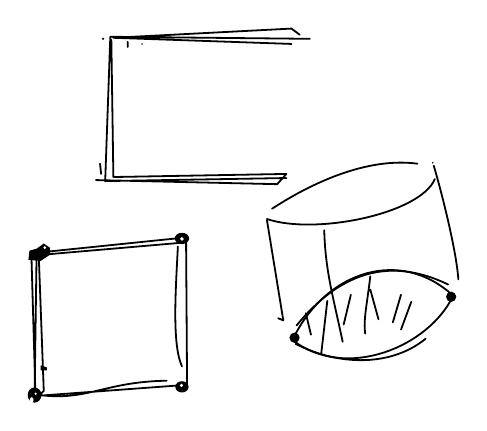
\begin{tikzpicture}[x=.013cm,y=-.013cm,line width=.65pt,line cap=round,line join=round]
\draw (1805,608)--(1610,606)--(1605,747)--(1782,744)
 (1795,604)--(1787,598)--(1613,607)--(1787,613)
 (1611,609)--(1613,743) (1596,746)--(1773,750)--(1782,740)--(1614,743);
\fill (1603,608) circle[radius=1.2] (1641,613) circle[radius=.8];
\draw (1627,611)--(1627,616) (1600,730)--(1601,740);
\draw (1538,817)--(1684,802)--(1685,946)--(1536,957)--cycle
 (1543,819)--(1682,807) (1533,822)--(1537,960)--(1545,952)--(1540,817)
 (1676,811)..controls(1674,852)and(1670,906)..(1680,928)
 (1541,956)..controls(1588,962)and(1604,943)..(1665,942);
\fill (1531,815)--(1538,813)--(1545,808)--(1551,812)--(1551,819)
 --(1542,825)--(1530,824)--cycle;
\fill (1680,803) ellipse[x radius=7,y radius=5.5];
\fill (1680,948) ellipse[x radius=6.5,y radius=5.5];
\fill (1536,956) ellipse[x radius=6.7,y radius=7.4];
\fill[white] (1546,812) circle[radius=1.5]
 (1680,803.5) circle[radius=1.9] (1679.5,946.6) circle[radius=1.7]
 (1537.1,954.7) circle[radius=1.25];
\fill[white] (1533.2,960.8) ellipse[x radius=1.8,y radius=2.7];
\fill (1542,927)--(1548,929)--(1548,932)--(1542,932)--cycle;
\draw (1768,774)..controls(1814,744)and(1866,724)..(1910,730)
 (1763,784)..controls(1810,800)and(1913,779)..(1927,745)
 (1763,785)--(1779,883)--(1774,881) (1926,732)..controls(1932,752)and(1948,813)..(1950,843)
 (1819,795)..controls(1820,835)and(1828,861)..(1837,904);
\fill (1925,729) circle[radius=.9];
\draw (1789,900)..controls(1822,834)and(1894,812)..(1945,859)
 ..controls(1921,909)and(1841,942)..(1789,903);
\draw (1792,888)..controls(1832,839)and(1880,819)..(1940,848)
 (1791,906)..controls(1834,928)and(1885,928)..(1918,901);
\draw (1801,876)--(1806,897) (1822,864)--(1816,916) (1845,858)--(1838,887)
 (1864,840)..controls(1861,866)and(1857,883)..(1859,896)
 (1864,853)--(1872,882) (1894,858)--(1886,885) (1904,865)--(1894,892);
\fill (1790,900) circle[radius=5] (1943,860) circle[radius=5];
\end{tikzpicture}}

\[
\tikz[baseline=(markletters.base)]{
 \node[inner sep=0pt] (markletters) {\(\unsure{X_0|X_{\varnothing}}\qquad X_1\)};
 \draw[line width=.32pt] ([xshift=.75em,yshift=-.4em]markletters.west)
 ..controls ([xshift=1.4em,yshift=.5em]markletters.west) and ([xshift=-1.05em,yshift=.6em]markletters.east)
 ..([xshift=-1em,yshift=-.05em]markletters.east)
 ..controls ([xshift=-.95em,yshift=-.6em]markletters.east) and ([xshift=-.5em,yshift=-.5em]markletters.east)
 ..([xshift=-.1em,yshift=0em]markletters.east)
 ..controls ([xshift=.1em,yshift=.2em]markletters.east) and ([xshift=.15em,yshift=.2em]markletters.east)
 ..([xshift=.2em,yshift=-.1em]markletters.east);
 \draw[line width=.25pt] ([xshift=.35em,yshift=.02em]markletters.west)
 --([xshift=.72em,yshift=.5em]markletters.west);
 \draw[line width=.4pt] ([xshift=-.8em,yshift=.95em]markletters.east)
 --([xshift=-.78em,yshift=.85em]markletters.east);}
% The connecting trace and detached upper tick are not assigned an arrow
% or cancellation function. The crossed first index remains uncertain.
\]

\[
\bullet\quad O_1\subset\mathbb F_1\qquad
\deleted{\mathbb F}O_2\subset\mathbb F_2\quad\text{---}\quad O_n\subset
\tikz[baseline=(lastinclusionF.base)]{
 \node[inner sep=0pt] (lastinclusionF) {\(\mathbb F_n\)};
 \fill ([xshift=-.25em,yshift=.09em]lastinclusionF.north west) circle[radius=.023em];}
\]

\[
\tikz[baseline=(rightoverlay.base)]{
 \node[inner sep=0pt] (rightoverlay) {\(\unsure{\deleted{O}\hat{\mathbb F}|\deleted{\mathbb F}\hat O}\)};
 \draw[line width=.3pt] ([xshift=-.16em,yshift=-.1em]rightoverlay.south west)
 --([xshift=-.02em,yshift=.22em]rightoverlay.south west);}
 \subset\mathbb F
% Overlay order is uncertain. The low left slant is literal, with function unassigned.
\]

\[
\mathbb F_1\times\text{---}\,
\mathbin{\tikz[baseline=(tickcross.base)]{
 \node[inner sep=0pt] (tickcross) {\(\times\)};
 \draw[line width=.3pt] ([xshift=.12em,yshift=.36em]tickcross.north)
 ..controls ([xshift=.2em,yshift=.23em]tickcross.north) and ([xshift=.18em,yshift=.13em]tickcross.north)
 ..([xshift=.08em,yshift=.08em]tickcross.north);}}
\mathbb F_n
\mathbin{\tikz[baseline=(dotcross.base)]{
 \node[inner sep=0pt] (dotcross) {\(\times\)};
 \fill ([xshift=.12em,yshift=.12em]dotcross.north east) circle[radius=.45pt];}}
(-\,?)
% Detached curved tick above the second cross and dot above-right of the
% third cross are reproduced literally; their linguistic status is unknown.
\]

\[
(O_1,\mathbb F_1
\tikz[baseline=(pairclose.base)]{
 \node[inner sep=0pt] (pairclose) {\()\)};
 \draw[line width=.3pt] ([xshift=-.02em,yshift=.04em]pairclose.center)
 --([xshift=-.22em,yshift=-.2em]pairclose.center);}
\mathbin{*}(O_2,\mathbb F_2)\ 
\tikz[baseline=(pairdash.base)]{
 \node[inner sep=0pt] (pairdash) {\(\text{---}\)};
 \fill ([xshift=-.25em,yshift=.08em]pairdash.west) ellipse[x radius=.02em,y radius=.04em];}
\mathbin{*}
(\deleted{\unsure{O|0}}\unsure{O_3|O_n}\,\unsure{F_n|F_{n+1}|F_3})\,.
\]

\figure{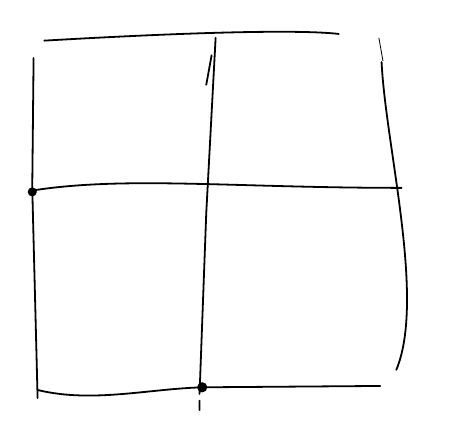
\begin{tikzpicture}[x=.017cm,y=-.017cm,line width=.65pt,line cap=round]
\draw (1374,1202)..controls(1460,1197)and(1559,1193)..(1594,1197)
 (1366,1215)--(1365,1312)--(1369,1469)
 (1365,1314)..controls(1435,1303)and(1515,1312)..(1641,1312)
 (1502,1200)--(1495,1331)--(1490,1466) (1490,1471)--(1490,1478)
 (1499,1213)--(1495,1235)
 (1369,1463)..controls(1410,1473)and(1452,1462)..(1493,1461)--(1625,1460)
 (1626,1218)..controls(1629,1281)and(1659,1395)..(1637,1448);
\draw[line width=.3pt] (1624,1200)--(1627,1217);
\fill (1365,1315) circle[radius=3.4] (1492,1461) circle[radius=3.8];
\end{tikzpicture}}

\[
(F\times I)\mathbin{\amalg}_{\unsure{\deleted{O}\dot{\mathbb F}|\dot B}\times I}
\deleted{O}\hat{\mathbb F}
% The final overlay follows the first candidate of the earlier order doubt.
% The small subscript composite retains a separate B alternative.
\]
% archive sheet number: 3

\scanpage{5}

\diagram{\begin{tikzcd}[ampersand replacement=\&,column sep=.7em]
{\mathbb Z[\mathbb F_{\unsure{n-2|n\,2|n-1}}]}
\& {\begin{tikzpicture}[baseline=-.15em,x=.45em,y=.45em,line width=.45pt]
\draw (.7,.7)..controls(-.1,.45)and(-.15,-.1)..(.55,-.5);
\draw (.45,.05)--(1.65,.05);
\end{tikzpicture}}
\& {\mathbb Z[\mathbb F_{n-1}]}
\& {\mathbb Z[F_n]}\arrow[l,"{t_n-s_n}"]
\& {\mathbb Z[\mathbb F_{n+1}]}\arrow[l]
\& {\begin{tikzpicture}[baseline=-.3ex,x=.5em,y=.5em,line width=.8pt]
\draw (0,.15)--(.65,.15);
\draw (.43,.55)--(.43,-.3)--(.7,-.3);
\draw (0,0)--(0,.3);
\end{tikzpicture}}
\end{tikzcd}}
% The first connector has an open curved head separated from its shaft.
% The middle left-arrow label is below the shaft, as in C's equivalent syntax.
% The terminal cross-like trace has no securely assigned lexical/algebraic value.
\figure{\begin{tikzpicture}[x=1em,y=1em,line width=.4pt,line cap=round]
\draw (0,.35)..controls(.04,.08)and(.2,-.05)..(.3,-.12);
\draw (.35,-.16)--(.4,-.18);
\draw (.48,-.21)--(.6,-.23);
\draw (1.1,.06)--(1.2,.13);
\draw (1.28,.2)--(1.48,.32);
\end{tikzpicture}}
% Detached curved traces below the chain; uncertain function, no word assigned.

\[
\begin{aligned}
D_n&\longrightarrow X &\quad&\deleted{D_n}\,\raisebox{1.1ex}{\(\cdot\)}\\
\bigl\{x&\in F_n && =
\end{aligned}
\]

% The source's first and last small arguments lack a separate opening parenthesis.
% The square-ended low bracket occupies source [265,630,588,658], below only the left part.
\figure{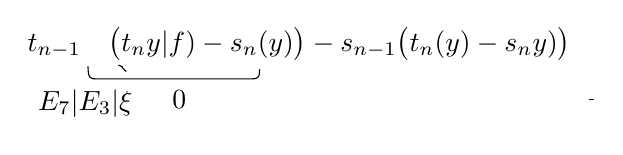
\begin{tikzpicture}[line width=.4pt]
\node[anchor=west,inner sep=0pt] (eq) at (0,0)
 {$t_{n-1}\quad\bigl(t_n\unsure{y|f})-s_n(y)\bigr)-s_{n-1}\bigl(t_n(y)-s_n y)\bigr)$};
\draw ([xshift=2.2em,yshift=-.8em]eq.west)
 .. controls ([xshift=2.2em,yshift=-1.25em]eq.west) and ([xshift=2.3em,yshift=-1.25em]eq.west)
 .. ([xshift=2.5em,yshift=-1.25em]eq.west)
 -- ([xshift=8.1em,yshift=-1.25em]eq.west)
 .. controls ([xshift=8.4em,yshift=-1.25em]eq.west) and ([xshift=8.4em,yshift=-1.15em]eq.west)
 .. ([xshift=8.4em,yshift=-.9em]eq.west);
\node at ([xshift=5.5em,yshift=-2em]eq.west) {$0$};
\draw ([xshift=3.3em,yshift=-.75em]eq.west)
 --([xshift=3.46em,yshift=-.82em]eq.west);
\draw ([xshift=3.42em,yshift=-.83em]eq.west)
 --([xshift=3.58em,yshift=-.98em]eq.west);
\node at ([xshift=2.1em,yshift=-2.15em]eq.west) {$\unsure{E_7|E_3|\xi}$};
% A short detached ink dash at source [1168,696,1180,705].
\draw ([xshift=20.3em,yshift=-2em]eq.west)--([xshift=20.48em,yshift=-2em]eq.west);
\end{tikzpicture}}

\[
\begin{array}{cc}
\underset{\smile}{F}_0 & F_1\\[.6em]
F'_0 & \mathbb F'_1\\
\unsure{1|\prime}&
\end{array}
\]
\diagram{\begin{tikzcd}[ampersand replacement=\&,column sep=1.7em,row sep=1.3ex]
\&\& \unsure{s|f}\&t\arrow[l]\\
{\substack{\exists\,\deleted{u}s,u'\\s'}} \&
 f(s)\arrow[l] \& f_0(s) \& f_0(t)\arrow[l]
\end{tikzcd}}

\begin{flushright}
\begin{minipage}{.74\linewidth}
\(\bigl(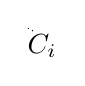
\begin{tikzpicture}[baseline=-.55ex,x=1em,y=1em]
\node[inner sep=0pt] at (0,0) {$C_i$};
\fill (-.5,.65) circle (.025);
\fill (-.35,.57) circle (.025);
\end{tikzpicture}\bigr)\quad\forall w'\in\mathbb F'_i,\)
\deleted{si on \unsure{retient|retire}} \(\deleted{s}\exists w\in F_i.\) tel que
\(f(w)\sim w'\). De plus si \(i\geq1\), On peut
\par\noindent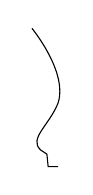
\begin{tikzpicture}[baseline=-2.3em,x=.45em,y=.5em,line width=.4pt]
\draw (0,5)..controls(1.7,3)and(2.6,1)..(2.1,-.4)
 ..controls(1.4,-2)and(-.3,-3)..(.7,-3.8)--(1.2,-4.1)--(1.3,-5)--(2.1,-5);
\end{tikzpicture}\begin{minipage}{.89\linewidth}
se donner d'avance \(u_{\unsure{i|i-1}}=s_i(w)\), \inserted{\(v_i=\)}\(t_i(w)\),
\inserted{de \(F_{i-1}\)} soumis aux seules conditions \deleted{de} que
\(f(u_{\unsure{\cdot|i|1}})=u'_{\unsure{i|1}}\), \inserted{\unsure{rp|resp}}
\(\unsure{g|f}(v_i)=v'_i\)
et, \deleted{de} plus, si \(i-1\geq1\) i.e \(i\geq2\), \deleted{que}
\(s(u)=s(v),\ t(u)\unsure{\equiv|=}t(v)\)
\end{minipage}

(NB on n'exige pas que \(g(u)=u'\))
\end{minipage}
\end{flushright}
% The two points above-left of C are literal detached ink, not an assigned accent.
% The later v/v' subscripts retain the i/1 doubt first marked on u'.
% The NB function shares the g/f uncertainty of the preceding equality;
% its use of g is the first candidate, not a separate resolution of that form.

\[
\begin{aligned}
\unsure{\Xi|E}_0\quad\text{\textcircled{\(\unsure{\mathrm b)|\mathrm a)}\)}}\quad&
\forall s'\in F'_0,\quad \exists s\in\mathbb F_0,\ u\in\mathbb F'_1,\quad
f_0(s)\xrightarrow{u}s'\\[-.1em]
&\hspace{4em}\deleted{\pi_0(f)\ \unsure{\text{surj}}}\quad
-\pi_0(f)\ \text{\uuline{surj}}\\
\mathrm b)\quad&
\forall s,t\in F_0,\quad
\underset{\substack{\rotatebox{-90}{\(\in\)}\\F'_1}}{u'}:f_0(s)\longrightarrow f_0(t),\\
&\exists u\in\mathbb F_1,\quad u:s\mathbin{-}t\qquad\pi_0(f)\ \text{inj.}
\end{aligned}
\]

\[
\begin{aligned}
\Xi_1\quad\text{\textcircled{\(\mathrm b')\)}}\quad&
\forall s,t\in\mathbb F_0,\quad
\underset{\substack{\rotatebox{-90}{\(\in\)}\\F'_1}}{u'}:
 f_0(s)\mathbin{-} f_0(t),\\
&\exists u\in F_1,\quad u:s\mathbin{-}t,\quad
 f(u)\mathrel{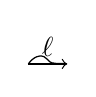
\begin{tikzpicture}[baseline=-.4ex,x=.35em,y=.35em,line width=.45pt]
\draw[->] (0,0)--(4,0);
\draw (0,0)..controls(.7,1.0)and(1.6,1.0)..(2,.45)
 ..controls(2.5,-.25)and(3.4,.2)..(4,0);
\node at (2,1.8) {$\ell$};
\end{tikzpicture}}u' \\
&\deleted{\unsure{w|\exists\,w|u}\in F_2}\\
&\pi_0(f)\ \text{inj. et }\text{\uuline{\(\pi_1(f)\) surj}}
\end{aligned}
\]
% The wavy stroke is traced across the shaft. Xi_1 follows the first candidate
% of the Xi/E uncertainty marked at the preceding level; E_2 below has a clear stem.

\[
\begin{aligned}
\mathrm c)\quad&
\deleted{\forall s,t\in\mathbb F_0,}\ u,v\in\unsure{F|\mathbb F}_1\quad
\begin{gathered}s_i(u)=s_1(v),\\[-.2em] t_1(u)=t_1(v)\end{gathered},\\
&\text{et }\underset{\substack{\rotatebox{-90}{\(\in\)}\\\mathbb F'_2}}{w'}:
 f(u)\longrightarrow f(v),\quad
 \exists\underset{\substack{\rotatebox{-90}{\(\in\)}\\\mathbb F_2}}{w}:
 \deleted{\unsure{f_1|f}}u\mathbin{-}v\\
&\pi_{\unsure{f|1}}(f)\ \text{inj.}
\end{aligned}
\]
% Source [470,1372,583,1508]: two arrows have separate endpoints, with gaps on both sides.
\figure{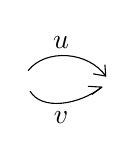
\begin{tikzpicture}[x=1.4em,y=1em,line width=.4pt,line cap=round,line join=round]
\draw (-1,.2)..controls(-.55,1)and(.55,.9)..(1,0);
\draw (.68,.08)--(1,0)--(.98,.4);
\draw (-.95,-.55)..controls(-.65,-1.25)and(.3,-1.05)..(.9,-.4);
\draw (.55,-.37)--(.9,-.4)--(.65,-.66);
\node at (-.15,1.2) {$u$};
\node at (-.15,-1.5) {$v$};
\end{tikzpicture}}

\[
\begin{aligned}
E_2\quad\text{\textcircled{\(\mathrm c'\)}}\quad&
\forall(u,v)\in\mathbb F_1,\quad
\begin{gathered}s_1(u)=s_1(v)\\[-.2em] t_1(u)\mathbin{-}t_1(v)\end{gathered}
\quad\text{et }\underset{\substack{\rotatebox{-90}{\(\in\)}\\\mathbb F'_2}}{w'}:
 f(u)\mathbin{-}f(v),\\
&\exists\underset{\substack{\rotatebox{-90}{\(\in\)}\\\mathbb F_2}}{w}:u\longrightarrow v\ 
 \mathord{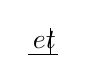
\begin{tikzpicture}[baseline=(oldet.base),line width=.4pt]
\node[inner sep=0pt] (oldet) {\(\deleted{\text{et}}\)};
\draw ([xshift=-.15em,yshift=-.2em]oldet.south west)
 --([xshift=.05em,yshift=-.2em]oldet.south east);
\draw ([xshift=-.2em,yshift=.1em]oldet.north east)
 --([xshift=-.2em,yshift=-.22em]oldet.south east);
\end{tikzpicture}}\ \text{tel que}\\
&w'\sim f(w)
\end{aligned}
\]
% Source [1981,1363,2342,1520]: asymmetric rounded grouping stroke, without a central brace peak.
\figure{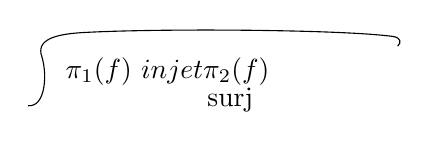
\begin{tikzpicture}[x=1em,y=1em,line width=.4pt]
\node[anchor=west] at (0,0) {$\pi_1(f)\ \text{inj et }\pi_2(f)$};
\node at (6.3,-1.05) {surj};
\draw (-1,-1.25)..controls(-.4,-1.3)and(-.3,-.2)..(-.5,.5)
 ..controls(-.75,1.15)and(0,1.35)..(1.1,1.4)
 ..controls(4,1.55)and(10.4,1.5)..(12.2,1.25)
 ..controls(12.45,1.2)and(12.5,1.05)..(12.35,.9);
\end{tikzpicture}}
% Source [1109,1538,1203,1657]: separated arc endpoints; lower right return; three detached dots.
% The vertical arrow passes between the w and its prime, not to the right of the prime.
\figure{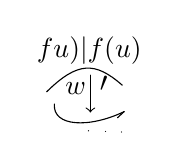
\begin{tikzpicture}[x=1.4em,y=1.1em,line width=.4pt,line cap=round,line join=round]
\draw (-1,0)..controls(-.2,1)and(.25,1)..(.95,.22);
\draw (-.8,-.4)..controls(-.85,-1.15)and(.1,-1.2)..(1,-.65);
\draw (1,-.65)--(.83,-.85);
\node at (.1,1.35) {$\unsure{fu)|f(u)}$};
\node at (-.25,.12) {$w$};
\node at (.47,.25) {$\prime$};
\draw[->] (.13,.55)--(.13,-.68);
\fill (.08,-1.28) circle (.025em);
\fill (.52,-1.3) circle (.022em);
\fill (.93,-1.32) circle (.022em);
\end{tikzpicture}}
% archive sheet number: 4
% Pale rotated background impressions are present; no additional word was recoverable securely.

\scanpage{6}

% Main 01: reused typescript strip, running bottom to top at the left.
\[
\underline{\mathrm B}=(\text{Gr-stacks})\qquad
\widehat{\underline{\mathrm B}}\qquad
\underline{\mathrm B}(\unsure{0|\mathrm O})^{\wedge}
\]
commutes not only with arbitrary projective limits, but equally with arbitrary direct limits, or what amountsto the same, that direct limits in the category (Gr-stacks) can be computed component-wise. (Here \(\underline{\mathrm B}(0)\) stands for the full subcategory of \(\underline{\mathrm B}\) formed by the basic objects \(\underline{\mathrm D}_n\), \(n\ \underline{\mathrm N}\) .)
% The repeated typed 0 uses the first candidate of the same retained 0/O doubt.

\handwritten{
% Main 02: the isolated D is doubled; the live indexed D is plain.
\[
\widetilde{\mathbb D}\qquad
\unsure{\mathscr N|N}\longmapsto
\overset{\deleted{\unsure{I_n|D_n}}}{\widetilde D_n}
\]

% Main 06: the lower leading relation is a new main-reader doubt.
\[
\begin{aligned}
&1+n\mathbin{.}2^1+\frac{n(n-1)}{2}\,2^2\ \text{---}\ +2^n\\
&\qquad\unsure{>|=}(1+2)^n=
\end{aligned}
\]

% Main 03: three distinct rightward shafts and heads.
% Main 04: the down arrow ends over n, with membership and I in the next cell.
\diagram{\begin{tikzcd}[ampersand replacement=\&,row sep=1.15em,column sep=.35em]
\widetilde D_{n'}\arrow[r,bend left=38]\arrow[r]\arrow[r,bend right=38]
 \&[1.65em] \widetilde D_n \& {}\\
 \& \widetilde D_n\arrow[d] \& {}\\
 \& n \& {\in\begin{tikzpicture}[baseline=(downI.base),x=1em,y=1em]
\node[anchor=base,inner sep=0pt] (downI) at (0,0) {$\mathbb I$};
% Literal detached triangular point above, slightly left of the I stems.
\fill (-.065,.93)--(-.025,1.005)--(.025,.945)--cycle;
\end{tikzpicture}}
\end{tikzcd}}

% Main 05: both upper I forms are doubled; the old qualifier remains uncertain.
\[
\begin{aligned}
d_n\in\widetilde D_n&\longrightarrow\deleted{N}\mathbb I
 &\qquad d_n&\longmapsto n\\
&\text{strictement}\\
&\text{croissante}\\
&\text{image \unsure{est|\(\subset\)}}\ \mathbb I_{\deleted{\unsure{\in n|<n}}\leq n}
\end{aligned}
\]

% Main 09 and 10: detached traces, preserved without assigned lexical meaning.
\figure{\begin{tikzpicture}[line width=.5pt,line cap=round,line join=round]
% Main 09: slight rise at the entry of the upper short trace.
\draw (0,0)..controls(.025,.025)and(.06,.02)..(.13,.015);
% Main 10: point above-left, uneven rule, weak interval, angular terminal return.
\fill (2.61,-1.15) circle[radius=.018];
\draw (2.68,-1.23)..controls(2.78,-1.21)and(2.89,-1.25)..(2.94,-1.25);
\draw[line width=.18pt] (2.94,-1.25)--(2.975,-1.25);
\draw (2.985,-1.25)--(3.005,-1.28)--(3.03,-1.25);
\end{tikzpicture}}

% Main 07: margin note written sideways; both membership arches open downward.
% First live eta/g/y and xi/f/x doubts govern the later repeated candidates.
% Local limits remain eta/y over the middle J, xi/x over the last J,
% and xi/x/f at the lower endpoint; the repeated xi and eta do not resolve them.
\margin{\resizebox{.99\marginparwidth}{!}{\begin{minipage}{17em}
\diagram{\begin{tikzcd}[ampersand replacement=\&,column sep=1.3em,row sep=.65em]
J_{n''}\arrow[r,"{\unsure{u_\eta|u_g|u_y}}"] \&
 {\overset{\substack{\eta\\\rotatebox{-90}{\(\in\)}}}{J}_{n'}}
 \arrow[r,"{\overset{\deleted{\unsure{u_\eta|u_g}}}{\unsure{u_\xi|u_f|u_x}}}"{inner sep=0pt,yshift=-.15em}]
 \arrow[dr,bend right=16,"{\unsure{u}}"{description,sloped,inner sep=0pt,fill=none}] \&
 {\overset{\substack{\xi\\\rotatebox{-90}{\(\in\)}}}{J}_{\deleted{\unsure{n'}}n}}\\
 \& \& \xi
\end{tikzcd}}
% Main 08: the two-bar equality has no written right member.
\(u_\xi u_\eta=\)
\end{minipage}}}
% The tentative diagonal u is centered on its bowed shaft, without a white backing.

% Main 11: this separate map precedes the x/y array in page order.
\[
\widetilde D_{n'}\longrightarrow\widetilde D_n
\]

% Main 12: one canceled left cluster, no separately surviving live connector.
% The common live D is at the intervening level between the two memberships.
\diagram{\begin{tikzcd}[ampersand replacement=\&,column sep=1.25em,row sep=.35em]
x'' \& {<} \& x'\arrow[dd,dash] \& {\in} \& {}\\
\deleted{\unsure{\downarrow|I|=}} \& \&
 |[xshift=-.35em]|{\begin{tikzpicture}[baseline=0pt]
\fill (0,0) circle[radius=.025em];
\end{tikzpicture}}
 \& \& {\overset{\deleted{D}}{\widetilde D_n}}\\
y'' \& {<} \& y'\arrow[d,dash] \& {\in} \& {}\\
{} \& \& n' \& \&
\end{tikzcd}}
\figure{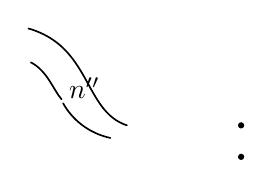
\begin{tikzpicture}[line width=.6pt,line cap=round]
% The upper arc crosses n'', which is not a free array cell.
\node[inner sep=0pt] at (.71,-.01) {$n''$};
\draw (0,.75)..controls(.8,.52)and(.7,-.3)..(1.25,-.48);
% The lower arc has a short real gap part way down.
\draw (.03,.32)..controls(.24,.21)and(.31,-.02)..(.42,-.15);
\draw (.44,-.20)..controls(.55,-.40)and(.76,-.58)..(1.04,-.64);
\fill (2.7,-.48) circle[radius=.04] (2.7,-.88) circle[radius=.04];
\end{tikzpicture}}

% Main 13: plain I, ens without a stop, and a detached point before n.
\(I\) ens ordonné

\(\mathord{\begin{tikzpicture}[baseline=-.15ex,x=1em,y=1em]
\fill (0,0) circle[radius=.03];
\end{tikzpicture}}\quad n\longmapsto\widetilde D_n\) famille d'ens ordonnés \unsure{,|;}

% Main 14: resolved old phi; a literal oblique mark above-left of the live label.
% Main 15: plain image I with a separate point below-left of its stem.
\[
\widetilde D_n\xrightarrow{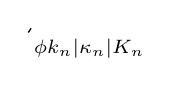
\begin{tikzpicture}[baseline=(maplabel.base),line width=.45pt]
\node[inner sep=0pt] (maplabel) {$\scriptstyle\deleted{\phi}\unsure{k_n|\kappa_n|K_n}$};
\draw ([xshift=-.18em,yshift=.22em]maplabel.north west)
 --([xshift=-.08em,yshift=.37em]maplabel.north west);
\end{tikzpicture}}I\qquad
\text{str. croiss.}\quad\text{image}\quad
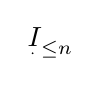
\begin{tikzpicture}[baseline=(imageI.base),x=1em,y=1em]
\node[anchor=base,inner sep=0pt] (imageI) at (0,0) {$I$};
\node[anchor=base west,inner sep=0pt] at (.2,-.3) {$\scriptstyle\leq n$};
\fill (-.08,-.24) circle[radius=.035];
\end{tikzpicture}
\]

% Main 16: the opening through K is canceled; the following capital Soit is live.
Si \(n'\leq n\), \deleted{\unsure{Soit|Sinon} l'ens \(K\)} Soit
% Main 17: left-aligned two-level definition, with a point above-left of vertical =.
\[
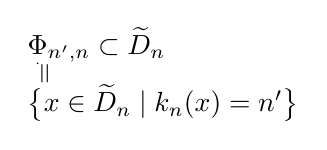
\begin{tikzpicture}[x=1em,y=1em]
\node[anchor=west,inner sep=0pt] at (0,0) {$\Phi_{n',n}\subset\widetilde D_n$};
\node[inner sep=0pt] (subseteq) at (.7,-1.05) {\rotatebox{90}{\(=\)}};
\fill (.38,-.66) circle[radius=.035];
\node[anchor=west,inner sep=0pt] at (0,-2.1)
 {$\bigl\{x\in\widetilde D_n\mid k_n(x)=n'\bigr\}$};
\end{tikzpicture}
\]
% The clean k_n carries the earlier k/kappa/K doubt; it is not a new resolution.

% Main 18: the prime and final comma both belong to the canceled phrase.
\deleted{Soit \(x\in\Phi_{n'},\)}

% Main 19: the old D group and the live B alphabet retain their ordered alternatives.
Considérons l'ens \deleted{\(\unsure{\widetilde D_{n'}|D_n}\)}\(\unsure{B|\mathbb B|\mathscr B}\)

% Main 20: plain F_0, doubled F_1 and F_2; four literal leftward arrow paths.
\diagram{\begin{tikzcd}[ampersand replacement=\&,column sep=.15em]
F_0 \& {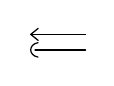
\begin{tikzpicture}[baseline=-.3ex,x=.9em,y=1em,line width=.45pt,line cap=round,line join=round]
% Upper first arrow: head joined to shaft.
\draw (2.2,.28)--(0,.28);
\draw (.3,.5)--(0,.28)--(.3,.06);
% Lower first arrow: curved left head, with a white gap before the shaft.
\draw (.29,-.02)..controls(-.1,-.08)and(-.1,-.48)..(.29,-.54);
\draw (.17,-.28)--(2.2,-.28);
\end{tikzpicture}} \& \mathbb F_1
 \& {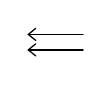
\begin{tikzpicture}[baseline=-.3ex,x=.9em,y=1em,line width=.45pt,line cap=round,line join=round]
% Both second-pair heads meet their shafts.
\draw (2.2,.28)--(0,.28);
\draw (.3,.5)--(0,.28)--(.3,.06);
\draw (2.2,-.28)--(0,-.28);
\draw (.3,-.06)--(0,-.28)--(.3,-.5);
\end{tikzpicture}} \& \mathbb F_2
\end{tikzcd}}

% Main 21: B's literal open contour, detached x, inward upper head, lower returns.
\figure{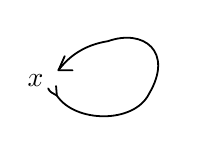
\begin{tikzpicture}[line width=.65pt,line cap=round,line join=round]
\node[inner sep=0pt] at (-.27,0) {$x$};
\draw (0,-.19)..controls(.23,-.54)and(.98,-.55)..(1.17,-.17)
 ..controls(1.49,.37)and(1.10,.66)..(.65,.50)
 ..controls(.33,.45)and(.14,.29)..(.02,.13);
\draw (.02,.13)--(.20,.13) (.02,.13)--(.10,.31);
\draw (0,-.19)--(-.01,-.07);
\draw (0,-.19)..controls(-.05,-.16)and(-.09,-.15)..(-.11,-.10);
\end{tikzpicture}}

% Main 22: headless vertical connector; a detached point below-left of the y prime.
\diagram{\begin{tikzcd}[ampersand replacement=\&,row sep=1.1em]
x'\arrow[d,dash]\\
{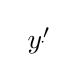
\begin{tikzpicture}[baseline=(footy.base),x=1em,y=1em]
\node[anchor=base,inner sep=0pt] (footy) at (0,0) {$y$};
\node[anchor=base,inner sep=0pt] at (.4,.35) {$\scriptstyle\prime$};
\fill (.28,.23) circle[radius=.035];
\end{tikzpicture}}
\end{tikzcd}}

% Main 23: three filled points, explicit upper arrow wings, disconnected low segment.
\figure{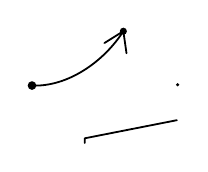
\begin{tikzpicture}[line width=.65pt,line cap=round,line join=round]
\fill (0,.15) circle[radius=.055];
\draw (0,.15)..controls(.45,.13)and(.91,.45)..(1.16,.84);
\draw (.92,.69)--(1.16,.84)--(1.20,.56);
\fill (1.16,.84) circle[radius=.045] (1.85,.16) circle[radius=.022];
\draw (.67,-.58)--(.67,-.52)--(1.84,-.29);
\end{tikzpicture}}

% Main 24: shallow broken V; the right arm itself has a second real interruption.
\figure{\begin{tikzpicture}[line width=.5pt,line cap=round]
\draw (0,.05)--(.07,0);
\draw (.11,.005)--(.145,.018);
\draw (.166,.027)--(.2,.04);
\end{tikzpicture}}

% Main 25: pi_0 and the written abbreviation/punctuation remain literal.
\[
\begin{aligned}
\pi_0(F_*,x)&=\text{ens des classes d'hom.topie. des}\\
&\phantom{=}\text{lacets en }x
\end{aligned}
\]
}% end handwriting
% archive sheet number: 5

\scanpage{7}
\mspage{1}

% This entirely handwritten page has no handwriting envelope (briefv06).
% Main 01: certain accent, unresolved direction; two quotation ticks each side.
Soit \(M\) une catégorie (``\unsure{modèles|modéles}''). On suppose

% Main 02: accent direction remains uncertain; no point after monomorphique.
(i) Toute \unsure{flèche|fléche} de \(M\) est monomorphique

% Main 03: abbreviated old word, uncertain old stop, raised end without stop.
(ii) Tout \deleted{\unsure{autom|autom.}}\inserted{end} d'un élément de \(M\) est l'identité.

% Main 04: the reduced internal strokes do not resolve par.
Ex : \(M\) une catégorie définie \unsure{par} un ensemble ordonné

% Main 05: quotation ticks and a real blank, without a hyphen, in sous objets.
% Main 06: no point follows the terminal tilded D of the identification.
Pour tout \(D\in\mathrm{Ob}\,M\), soit \(\widetilde D\) l'ensemble (ordonné par ``inclusion'') des sous objets de \(D\). On identifie \(D\) au plus grand élément de \(\widetilde D\)

Soient \(D',D\in\mathrm{Ob}\,M\), alors l'application
% Main 07: a literal two-row map; M belongs under the final m of Hom.
% Lower u is indented; its barred shaft starts farther left and runs longer.
% The star is far left between row levels; the upper target has no comma.
\diagram{\begin{tikzcd}[ampersand replacement=\&,row sep=0pt,column sep=0pt]
{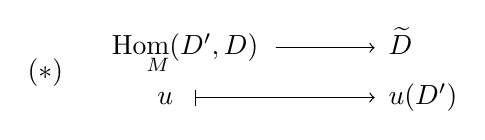
\begin{tikzpicture}[x=1em,y=1em,line width=.45pt,
 line cap=round,line join=round]
\node[anchor=base west,inner sep=0pt,outer sep=0pt] (homHo)
 at (0,0) {$\mathrm{Ho}$};
\node[anchor=base west,inner sep=0pt,outer sep=0pt] (homLast)
 at (homHo.base east) {$\mathrm m$};
\node[anchor=base west,inner sep=0pt,outer sep=0pt] (homArgs)
 at (homLast.base east) {$(D',D)$};
\node[anchor=north,inner sep=0pt,outer sep=0pt]
 at ([yshift=-.12em]homLast.south) {$\scriptstyle M$};
\node[anchor=base west,inner sep=0pt,outer sep=0pt]
 at (10,0) {$\widetilde D$};
\draw[->] ([xshift=.65em,yshift=.25em]homArgs.base east)--(9.5,.25);
\node[anchor=base west,inner sep=0pt,outer sep=0pt]
 at (1.65,-1.8) {$u$};
\draw[|->] (3,-1.55)--(9.5,-1.55);
\node[anchor=base west,inner sep=0pt,outer sep=0pt]
 at (10,-1.8) {$u(D')$};
\node[inner sep=0pt,outer sep=0pt] at (-2.4,-.65) {$(\ast)$};
\end{tikzpicture}}
\end{tikzcd}}
% Main 08: mixed first enclosure retained ahead of the two matched alternatives.
% Main 09: ens has no stop; the canceled de remains low-confidence;
% Phi is resolved, and inserted M- attaches before isomorphes.
est injective par \unsure{(i]|[i]|(i)}(ii), son image est formée de l'ens \deleted{\unsure{de}}
\(\Phi_{D'}(D)\subset\widetilde D\)
des sous-objets \(\Delta\) de \(D\) qui sont \inserted{\(M\)-}isomorphes à \(D'\).

\deleted{Soit \(K\) un ens. ordonné}

% Main 10--13 and 26: plain live N, deleted I, interlinear preordonne;
% the inserted sentence has only ordonne underlined; preceding M has its point.
Soit \(N\)\deleted{\(I\)} l'ens \inserted{préordonné} des classes d'isom. d'objets de \(M\). \inserted{Il est en fait \uline{ordonné}, grâce à (ii).}
% Main 14--18: unresolved forall/H, doubled N, canceled e/s, old D and live M;
% a raised star over n, and the first isom without a stop.
Pour \(\unsure{\forall|\mathrm H}\ n\in\mathbb N\), un\deleted{\unsure{e|s}} objet \(D_n\) de \deleted{\(D\)}\(M\) de classe \(\overset{\ast}{n}\) est déterminé à isom unique près,
% Main 19: reduced a/colon cluster plus a separate low down-right stroke.
% The literal stroke is neither a character candidate nor a therefore sign.
\begin{tikzpicture}[baseline=(causecluster.base),x=1em,y=1em,
 line width=.45pt,line cap=round]
\node[anchor=base west,inner sep=0pt,outer sep=0pt] (causecluster)
 at (0,0) {\unsure{à|:}};
\draw ([xshift=.12em,yshift=-.4em]causecluster.south east)
 --([xshift=.25em,yshift=-.62em]causecluster.south east);
\end{tikzpicture} cause de (ii),
% Main 20--22: ens without a stop; plain tilde D_n equals doubled J_n;
% resolved defini and the second isom without a stop.
donc l'ens ordonné \(\widetilde D_n=\mathbb J_n\) est défini à isom unique près.
% Main 23: dotted plui remains the first candidate; comma and old une are deleted.
On a donc \deleted{\unsure{plui|plus}, une}\inserted{une} famille
% Main 24: the family is a separate display.
\[
(\mathbb J_n)_{n\in\mathbb N}
\]
% Main 25: retain the observed footer wording and punctuation.
d'ens ordonnés, indexés par l'ensemble ordonné \(\mathbb N\).
% archive sheet number: 6

\scanpage{8}
De plus, se rappelant la definition de
\[
 J_n=\widetilde D_n=\text{ens des sous-objet de }D_n
\]
on a, pour \(\unsure{\mathrm{H}|\forall} n\in\mathbb N\), une application canonique, strictement croissante
\[
 J_n\xrightarrow{\tau_n}\mathbb N \qquad\qquad
 \text{\(\tau_n\), application ``type}
\]
dont l'image est formée \deleted{des} de l'ens
\deleted{\(I_{\leq n}\) des} \tikz[baseline=.2ex]{\fill (0,0) circle (.025);}% detached point; no punctuation function assigned
\(\mathbb N_{\leq n}=\{n'\in\mathbb N\mid n'\leq n\}\).

Notons que chaque \(J_n\) a un plus grand élément, qui est ``\(D_n\) (en tant que \inserted{le} sous-objet maximal de \(D_n\)), et \unsure{que je|qu'\deleted{est}on|qu'\deleted{il}on|qu'\deleted{est}on y|qu'\deleted{il}on y} note \(d_n\). On a donc \inserted{(par (ii))}
\[
 \tau_n^{-1}(n)=\{d_n\}
\]
\deleted{Si \(n'\leq n\), alors pour tout \(x\in J_n\)}

Soient \(n,n'\in\mathbb N\), \deleted{\(\unsure{x\in J|x\in}\)}\deleted{\(x\in J_n,\ n'=\tau_n(x)\), on} \inserted{avec \(n'\leq n\)}
considérons \deleted{\unsure{via \(x\)|via \((x)\)}} \deleted{on a alors \unsure{une|un} application}
\[
 \begin{aligned}
 \mathrm{Hom}(\deleted{\unsure{O|D}}D_{n'},D_n)&\hookrightarrow \widetilde D_n=J_n\\
 u&\mkern2mu\longmapsto u(d_{n'})
 \end{aligned}
\]
qui est une bijection des \(\mathrm{Hom}\) sur l'ens \(\tau_n^{-1}(n')\), et considérons
\[
 \mathrm{Hom}(\deleted{\unsure{D|O}}D_{n'}^{\unsure{4|\ast}},D_n)
 \longrightarrow
 \mathrm{Hom}\bigl(\underset{\substack{\tikz{\draw(0,.08)--(0,0)--(.60,0)--(.60,.08);}\\ J_{n'}}}{\widetilde D_{n'}},\underset{\substack{\tikz{\draw(0,.08)--(0,0)--(.54,0)--(.54,.08);}\\J_n}}{\widetilde D_n}\bigr)
 \quad\raisebox{-3.5ex}{\tikz{\fill (0,.12) ellipse (.025 and .018);\fill (-.07,0) circle (.022);}}% detached points; no punctuation function assigned
\]
on en déduit une \deleted{bijec} application
\[
 \begin{aligned}
 % One uncertain physical relation: rotated simeq | rotated equals; literal strokes retained.
 \underset{\left[\begin{gathered}
   \unsure{\tikz[x=1em,y=1em,baseline=0pt]{
     \draw[line width=.35pt] (.12,.56) .. controls (.18,.37) and (-.08,.12) .. (.02,.03)
       .. controls (.07,-.02) and (.18,-.02) .. (.23,.03);
     \draw[line width=.35pt] (.43,.59)--(.43,.08);
     \fill (0,.61) circle (.025);}}\\
   \mathrm{Hom}(D_{n'},D_n)
 \end{gathered}\right]}{\tau_n^{-1}(n')}
 &\overset{\mathrm{def}}{=}
 \underset{\substack{\tikz{\draw(0,.07)--(0,0)--(.86,0)--(.86,.07);}\\\text{ens des}\\\text{éléments}\\\text{de \(J_n\) de}\\\text{type \(n'\)}}}{J_{n',n}\deleted{\unsure{(n')|(n)}}}
 \xrightarrow{\rho_{n,n'}}\mathrm{Hom}(J_{n'},J_n)\\
 &\hspace{7em}\text{ou}\quad \xi\longmapsto u_{\xi}^{n}
 \end{aligned}
\]
qui est injective, plus précisément on a la \unsure{commutativité|commutativite}
\diagram{\begin{tikzcd}[ampersand replacement=\&,column sep=large,execute at end picture={
 \draw ([xshift=.15em,yshift=-1em]\tikzcdmatrixname-1-1.south east)
 ..controls +(-1.1em,.6em) and +(-2.1em,0)..
 node[pos=.95,above,inner sep=.5pt,fill=white] {\(\scriptstyle\text{inclusion}\)}
 ([xshift=.45em,yshift=-1.45em]\tikzcdmatrixname-1-2.south)
 ..controls +(1.9em,-.04em) and +(-1.0em,-.60em)..([xshift=-1em,yshift=-.75em]\tikzcdmatrixname-1-3.south west);}]
 J_{n,n'} \arrow[r,"\rho_{n,n'}"]
 \& \mathrm{Hom}(J_{n'},J_n) \arrow[r,"u\mapsto u(d_{n'})"] \& J_n
\end{tikzcd}}
% archive sheet number: 7
